\documentclass[journal]{IEEEtran}
\usepackage[style=ieee]{biblatex}
\bibliography{references.bib}
\usepackage{amsmath}
\usepackage[none]{hyphenat}
\usepackage{tgschola}
\usepackage{authblk}
\usepackage{amssymb}
\usepackage{siunitx}
\usepackage{fixmath}
\usepackage{graphicx}
\graphicspath{{./images/}}

\setlength{\parskip}{3mm}
\setlength{\parindent}{0mm}
\usepackage{titlesec}
\titlespacing{\subsubsection}{0pt}{0cm}{0.1cm}

\begin{document}
\title{Applications of ML in investigating Ferromagnetic Transitions}

\author[1]{Gautameshwar S.\thanks{All authors have contributed equally.}}
\author[2]{Ashish Panigrahi}\affil[1,2]{School of Physical Sciences\\NISER, Bhubaneswar}%

\maketitle

\begin{abstract}
This is an abstract.
\end{abstract}

\section{Introduction}

\subsection{Motivation}

The motivation behind our project is to investigate applications of machine learning in determining parameters in physical systems which are usually difficult to do so via a numerical approach.
In this project, we will be focusing on the one-dimensional and two-dimensional Ising spin models consisting of spin-1/2 atoms with either spin-\( \uparrow \) or spin-\( \downarrow \).

This project is divided into two parts:

\begin{enumerate}
    \item Finding the coupling constant \( J \) of the one-dimensional spin lattice.
    \item Classifying the phase orderness of a two-dimensional lattice depending on if the lattice temperature is beyond a critical point.
\end{enumerate}

\section{Theory}

\section{Results}

\subsection{1D Ising Model}

The first problem we will attempt to solve using machine learning is how we can find the pattern of 2-body interaction of atoms in a given 1D spin lattice.
To get a flavor of what our objective is, consider the following:

You are given a spin configuration of a 50-atom long spin lattice in the form of a 1D array.
Each of these elements are either in spin up (+1) or spin down (-1).
Suppose we consider the atom at the 5th site and say this atom adds stability to our lattice if both the spins neighbouring to it has the same spin as itself.
By asserting such a statement, we have indirectly defined the energy of interaction between the $5^{th}$ atom and $6^{th}$, $7^{th}$ atoms.
This statement, translated into a physics equation, states:

\[ E_{system}=J_{5,6}.\sigma_5\sigma_6+J_{5,7}.\sigma_5\sigma_7\]

where \(J_{5,6}, J_{5,7}\) are the strength of interaction between the atoms in the subscript.
If we extend the same argument to every single ith atom in the lattice interacting with every jth atom, we get the generalised 2-body interaction energy relation: \[E_{model}=\sum_{i,j=1}^{50}J_{ij}.\sigma_i\sigma_j\]

Now, if we are just given one lattice configuration with an energy label defined as above, there are countless possible \(J_{ij}\) matrices that are a valid solution to our above lattice.
If we manage to get all \(2^{50}\) unique lattice configurations, then there is analytically only one solution for our \(J_{ij}\).
But if we have some finite number of such 1D lattices with a energy label, it is possible to find the pattern in the nature of interaction of an atom with the other atoms of the lattice using regularised machine learning models.

\subsubsection{Data generation}

We assume a lattice at high temperature since temperature doesnt affect the J matrix.
A random assignment of spins in an 50 atom array along with the calculation of energy label based on the interaction matrix J defined by:

\begin{equation*}
    J_{ij} = \left\{
        \begin{array}{ll}
            -1 & \mbox{if } i = j \pm 1\\
            0 & \mbox{otherwise}
        \end{array}
    \right.
\end{equation*}

\begin{figure}
    \centering
    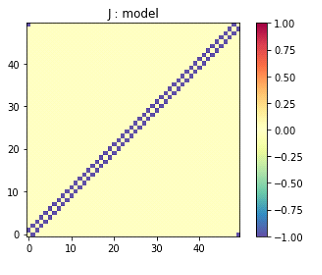
\includegraphics[scale=0.6]{J-model.png}
    \caption{J matrix for nearest neighbour interaction}
    \label{fig:j-matrix}
\end{figure}

\subsubsection{Unregularised Linear Regression}
We implement the \emph{Least Square Regression} model available in scikit-learn. The details provided below.
\begin{itemize}
    \item Parameter to train: \(J_{ij}\)
    \item Input variable: \(X_{ij}=\sigma_i\sigma_j\)
    \item Predicted Regression variable: \(E^n=X^n.J\), where $n$ is the $n^{th}$ lattice we input
    \item No of training lattices: N=10,000
    \item Loss function:
        \begin{equation*}
           \frac{1}{N} \sum_{n=1}^N(E_p^{(n)}-E_{label}^{(n)})^2
        \end{equation*}
    \item Score prediction method: Pearson's \(R^2\)
\end{itemize}

The results of linear regression turn out to be a perfect score for both training and testing data.

[code implementation of lsq]

The issue of overfitting is clearly seen in \cref{fig:overfit} if we plot the predicted $J$ matrix.

\begin{figure}[h!]
    \centering
    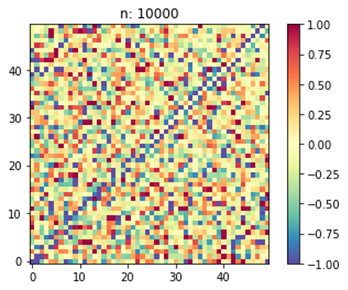
\includegraphics[scale=0.4]{overfitting.png}
    \caption{Overfitted $J$ matrix}
    \label{fig:overfit}
\end{figure}


[fig. of three instances of fitting the data]

[graph of score vs n]

The model overfits and produces perfect scores in both training and testing datasets after a certain size of input data because the statistical properties of our training and testing data becomes identical on large samples of lattices.
Thus overfitting gets away with it unattended!

\subsubsection{Regularised Lasso Regression}
We then implement the Lasso Regression model available in scikit-learn. The details provided below.
\begin{itemize}
    \item Parameter to train: \(J_{ij}\)
    \item Input variable: \(X_{ij}=\sigma_i\sigma_j\)
    \item Predicted Regression variable: \(E^n=X^n.J\), where n is the nth lattice we input
    \item Loss function: \(\lambda ||J||_1 + \frac{1}{N} \sum_{n=1}^N(E_p^{(n)}-E_{label}^{(n)})^2\)
    \item Score prediction method: Pearson's \(R^2\)
\end{itemize}

[code implementation of lasso]

The implementation of Lasso regression gave significant improvement in the overfitting issue.
For smaller datasets, we found a ``window of sweet-spot'' for \(\lambda\) in which the model accurately predicted the lattice interactions without any issue of overfitting.
For larger datasets, even a small regularisation \(\lambda\) yields an accurate prediction of our interaction matrix.

\begin{figure}[h!]
    \centering
    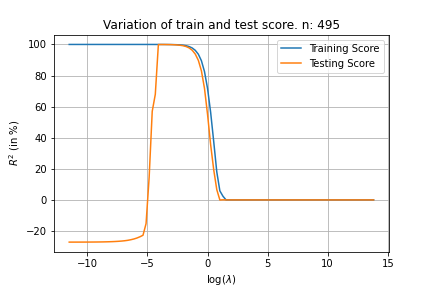
\includegraphics[scale=0.55]{lasso_n-495.png}
    \caption{Training and testing score as a function of \( \lambda \) (\( n=495 \)).}
\end{figure}


\begin{figure}[h!]
    \centering
    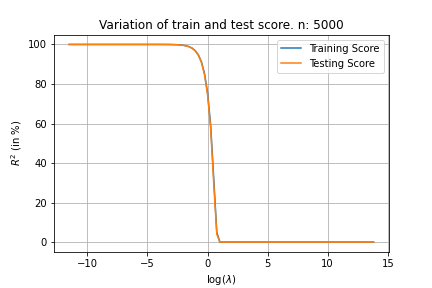
\includegraphics[scale=0.55]{lasso_n-5000.png}
    \caption{Training and testing score as a function of \( \lambda \) (\( n=5000 \)).}
\end{figure}


\subsubsection{Ridge Regression}
Finally we implement the Ridge Regression model available in scikit-learn. The details provided below.
\begin{itemize}
    \item Parameter to train: \(J_{ij}\)
    \item Input variable: \(X_{ij}=\sigma_i\sigma_j\)
    \item Predicted Regression variable: \(E^n=X^n.J\), where n is the nth lattice we input
    \item Loss function: \(\lambda ||J||_2 + \frac{1}{N} \sum_{n=1}^N(E_p^{(n)}-E_{label}^{(n)})^2\)
    \item Score prediction method: Pearson's \(R^2\)
\end{itemize}

[code implementation of ridge]

Unlike Lasso regression, Ridge did not offer any optimised regularisation \(\lambda\) for smaller datasets.
The model is seen to performed as poorly as LSQ.
However, on increasing the data size, our ridge performs better at predicting our interaction matrix without the issue of overfitting.

\begin{figure}[h!]
    \centering
    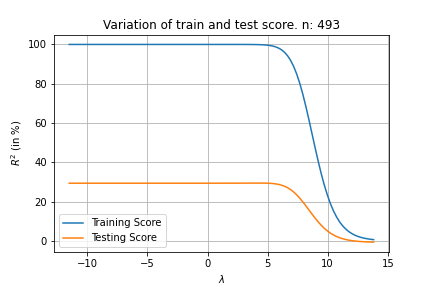
\includegraphics[scale=0.55]{ridge_n-493.png}
    \caption{Training and testing score as a function of \( \lambda \) (\( n=493 \)).}
\end{figure}

\begin{figure}[h!]
    \centering
    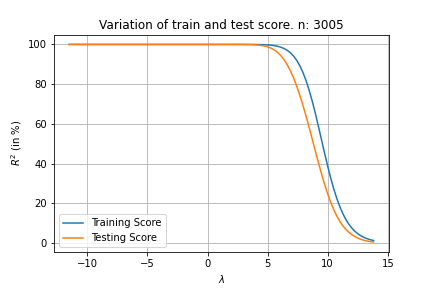
\includegraphics[scale=0.55]{ridge_n-3005.png}
    \caption{Training and testing score as a function of \( \lambda \) (\( n=3005 \)).}
\end{figure}



\subsubsection{Discussion on the results and further extension of our model}

We obtain contrastingly different results for Lasso and Ridge despite several similarities in them.
Both Ridge and Lasso don't like large values of \(||J||\) as it makes our data more sensitive to errors. They try to prefer $J$ with smaller ``slope'' than that with large one.
Thus, they regularise the overfitting issue efficiently.
But the optimisation of Lasso and ridge w.r.t LSQ is different.
It can be mathematically shown that:

\[J_{ridge}=\frac{J_{lsq}}{1+\lambda}\]

Thus, Ridge always scales the $J$ by the regularisation parameter.
Larger the \(\lambda\), more flat our ``slope'' becomes.
But even for large \(\lambda\), $J$ only approaches towards 0 asymptotically (close but never equal to 0).

\begin{figure}[h!]
    \centering
    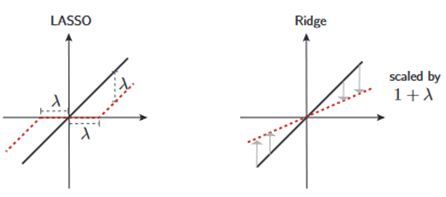
\includegraphics[scale=0.5]{ridge-vs-lasso.png}
    \caption{Visual schematic comparing Ridge and Lasso regression effects.}
\end{figure}

Lasso, on the other hand doesn't care about asymptotically reducing $J$.
As we increase \(\lambda\), the gap between the \(J_{lsq}\) and \(J_{lasso}\) where $J=0$ widens.
This results in more and more unimportant parts of our data being set to 0 (which we don't see in ridge).
Thus, for some specific \(\lambda\), we have exactly the unnecessary data set to 0, and the prominent parts of our ``slope'' $J$ intact.
This is the reason we see sweet spots that perfectly regularise by making the unnecessary overfitting to 0 and only retain the original model.
This is phenomenon is also referred to as ``sparse'' regression.

The Ridge model works at finding atom interaction beyond neighbours. We tested this by generating a data of lattices and labelling them with energy now defined by:

\begin{equation*}
    J_{ij} = \left\{
        \begin{array}{ll}
            -1 & \mbox{if } i = j \pm 1\\
            -0.5 & \mbox{if } i = j \pm 2\\
            0 & \mbox{otherwise}
        \end{array}
    \right.
\end{equation*}

[fig. of J model and predicted J]

[code result of scores ]

\subsection{2D Ising Training Data}
With our goal as to predict the ordered/disordered state of our lattice, we are in need of generating lots of Ising lattice data for each of the temperature steps about the critical temperature \(T_c\).
A 2D Ising lattice maintained at a temperature $T$ constantly fights between stabilising itself by lowering its energy and allowing itself to excite to a higher energy configuration due to the thermal agitation existing.
This is the result of the entropy of our lattice being minimised by establishing a statistical equilibrium between itself and the temperature reservoir in which it is existing.
The standard algorithm to simulate this statistical phenomenon is the Metropolis algorithm.

\subsubsection{The Metropolis Algorithm}
The goal of this algorithm is to find an equilibrium state for the two-dimensional spin lattice system at a particular temperature dictated by \(\beta\). It is achieved as follows:
\begin{enumerate}
    \item Begin with a random state \(\mu\) for the lattice configuration.
    \item Pick any random lattice site and flip the sign of the spin. We call this new state \(\nu\). What is the probability $P(\mu \rightarrow \nu)$ that we will accept this new state?
    \item If \(E_{\mu}>E_{\nu}\), then we set $P_{\nu \rightarrow \mu} = 1$ and thus by using the detailed balance equation we get $P_{\nu \rightarrow \mu} =e^{-\beta(E_{\nu}-E_{\mu})}$
    \item If $E_{\nu}>E_{\mu}$, then we set $P_{\mu \rightarrow \nu} = 1$ (i.e) with full probability, the spins gets flipped to a more stable configuration.
    \item Iterate step (1)-(4) as many times as required. Eventually we end up with an equilibrium state for large enough iterations
\end{enumerate}

The convergence for a solution is guaranteed for large enough iterations. It can be statistically shown that the relative error for the above Monte-Carlo goes as $\Delta E/E \approx 1/\sqrt{N}$ for large iterations $N$.

Our implementation of the Metropolis algorithm is done by defining a class 2D Ising model that has the following parameters and objects:

Input parameters while defining a class object of 2D ising model:
\begin{enumerate}
    \item \texttt{d}: Dimension of our 2D lattice. \texttt{dtype=int}
    \item \texttt{a}: Expected ratio of down spins to up spins in our randomly generated lattice
    \item \texttt{mfield}: Option to add the presence of an external magnetic field in our existing lattice.
\end{enumerate}

Objects in our 2D ising model class:
\begin{enumerate}
    \item \texttt{lattice}: Our randomly generated lattice (with 0 padded on the edge) on defining the 2D ising model object.
    \item \texttt{energy}: Computed energy of self.lattice
    \item \texttt{spin}: Computed net spin of self.lattice
\end{enumerate}

Functions in our 2D ising model class:
\begin{enumerate}
    \item \texttt{stable\_energy}: Function to compute the most stable energy configuration
    \item \texttt{get\_energy}: Function to compute the energy of \texttt{self.lattice}
    \item \texttt{flip\_check}: Inputs x,y co-ordinates, outputs the energy before and after flipping the spin at (x,y)
    \item \texttt{flip}: Inputs x,y co-ordinates, flips the spin at (x,y) of \texttt{self.lattice}
\end{enumerate}

We performed a numba implementation of our metropolis algorithm as it is extremely slow to perform iterations of order ~ 100,000 in a standard python executer. \\
Runtime of generating one 50x50 lattice after 100,000 metro iterations using a python executer: ~ 47 secs\\
Runtime of generating one 50x50 lattice after 100,000 metro iterations using Numba: ~ 0.18 secs

The data is organised as 10,000 Metro-generated lattices for one single temperature $T$. We have 20 such equally spaced temperatures in the range of $T$: 0.25-4 units.

Iteration plots of our Metropolis algorithm shows that our algorithm exhibits convergence for lower temperatures and fluctuates and becomes noisy with increase in temperature.
This is solely due to the fact that our system has an energy range for its likelihood to exist.
These energy states almost have equal likelihood due to high $T$, and this does not correspond to the fact that our algorithm misbehaves at those cases.
Spins usually do not converge since there are theoretically many spin configurations that might correspond to the same energy state.

[convergence plots for ordered, critical and disordered energies]

\subsection{2D Phase Transition Training}

\subsubsection{Labelling and implementing Random Forest Algorithm}

Now that we have generated our data, our objective now is to tell apart the ordered lattices from the disordered. The first task to achieve is to analytically find the critical temperature $T_c$ after which our lattices become disordered. This is given by \cite{onsager1944crystal}:

\[T_c=\frac{J}{\log(1+\sqrt{2})}\]

where $J$ is the strength of interaction of our atoms with its neighbours. With $J$=2 in our case, we have $T_c=2.26$.

\begin{figure}[h!]
    \centering
    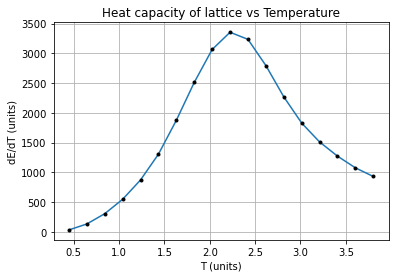
\includegraphics[scale=0.5]{cvst.png}
    \caption{Heat capacity vs temperature of lattice}
\end{figure}

\begin{figure}[h!]
    \centering
    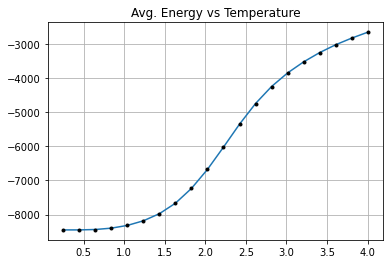
\includegraphics[scale=0.5]{evst.png}
    \caption{Energy vs temperature of lattice}
\end{figure}


Thus, all lattices above $T=2.26$ is labelled 0 (as disordered lattice) and the ones below are labelled 1 (as ordered lattice).
We further split our lattice into ordered, critical and disordered and proceed to only use the ordered and disordered lattices for training our model.
We reserve the set of critical lattices for verifying our models performance in critical region as it is expected to struggle to classify lattices in that region.
A better critical score means our model has learnt efficiently just from the ordered and disordered lattices on how to classify our lattices in the critical regime, along with the other regimes.

We implement a Random Forests classifier from scikit-learn as our training model for the above method due to the below reasons:

\begin{itemize}
    \item Our lattices are Monte-Carlo generated where our predictions are usually correlated. A spin flip in the initial stage of the Metropolis algorithm can result is an entirely new lattice configuration in the end. Thus weak classifiers such as decision trees and averaging several such models reduces the risk of choosing the wrong model (lowering the overall variance and bias).
    \item Ensemble methods such as RF reduces the risk of our model to rely on some greedy assumption or local search that may get stuck in a local extrema (quite common in Monte-Carlo data such as ours) and thus, it generates a better predicting model.
\end{itemize}

The Random Forests algorithm is implemented as follows:
\begin{itemize}
    \item Input variable: \(X=[x^i],x^i\in {X_{ordered}\bigcup X_{disordered}}\)
    \item Classifiers used: Decision Trees
    \item Hyperparameters used in tuning our optimal RF:
        \item \texttt{n\_estimators}: No. of decision trees in our forest.
        \item \texttt{min\_sample\_split}: No. of samples needed to split an internal node.
    \item Random sampling method: Bootstrap sampling
    \item Additional optimisation: Warm start=True. This ensures that you add estimators without fitting a whole new forest every time.
    \item Score prediction method for ordered and disordered samples: OOB estimators
    \item Score prediction method for critical samples: mean accuracy score (inbuilt score function in our training model)
\end{itemize}

The hyperparameter \texttt{min\_sample\_split} has two extremes: coarse and fine.
Increasing the above hyperparameter makes our forest much coarser.

The results obtained by Mehta \emph{et al.} \cite{2019} shows a poor performance in the critical samples though almost perfect for ordered and disordered samples. In the critical samples, vanilla RF gave a best accuracy of 69.2\% for coarse trees (leaf size: 10,000) compared to a accuracy score of 83.1\% for fine trees (leaf size: 2) at 100 estimators each.

\begin{figure}[h!]
    \centering
    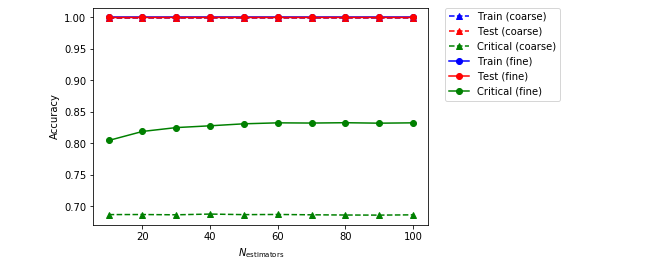
\includegraphics[scale=0.45]{mehta.png}
    \caption{Scores for various phases obtained in \cite{2019}.}
\end{figure}


\subsubsection{Improving the algorithm: Transductive Approach}
Given that we see the fact our model struggles in the critical region, we expect a deeper learning in the critical region will help our model get over the poor performance.
We implemented this idea into our random by introducing a transduction in our model by weighing the lattices closer to the critical regime more than the ones far from it.
Since scikit-learn does not have the option to add sample weight as an input, we performed data cloning so that our random forest encounters these samples more and trains more on them.
This simple hack will aid our algorithm to pick features more prominent in the critical region and by this emphasis, it trains deep in those features.
It also lowers the priority of features present in completely ordered/disordered lattices since they don’t play as important of a role as the lattices that are in the neighbourhood of the critical point.

[transduction graf]

Results of our modified Random Forests are as follows,

\begin{figure}[h!]
    \centering
    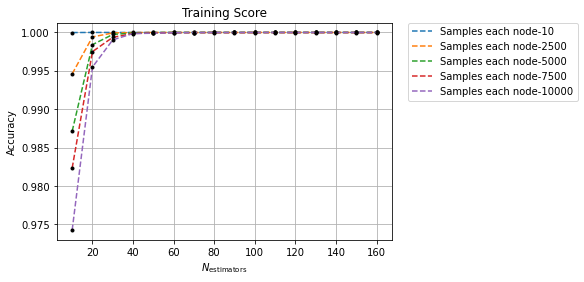
\includegraphics[scale=0.45]{train-score.png}
    \caption{Scores for training datasets obtained as a function of \( N_{\text{estimators}} \).}
\end{figure}

\begin{figure}[h!]
    \centering
    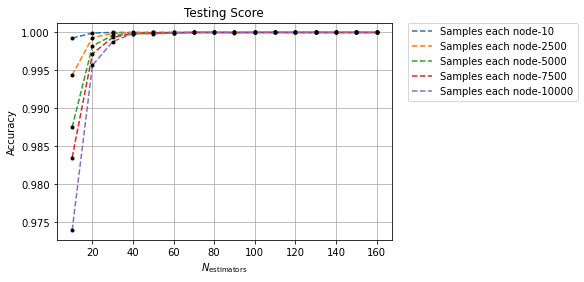
\includegraphics[scale=0.45]{test-score.png}
    \caption{Scores for testing datasets obtained as a function of \( N_{\text{estimators}} \).}
\end{figure}

\begin{figure}[h!]
    \centering
    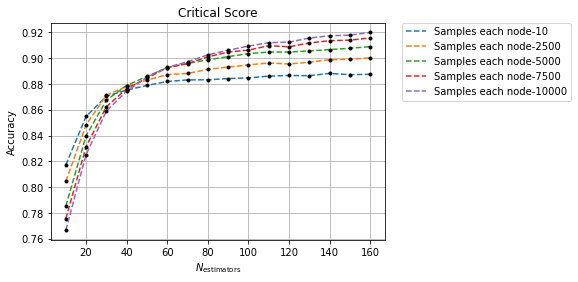
\includegraphics[scale=0.45]{critical-score.png}
    \caption{Scores for the critical phases obtained as a function of \( N_{\text{estimators}} \).}
\end{figure}

The results show an increase in the accuracy of the classification of critical samples compared to vanilla RF. Interestingly, by emphasising on samples closer to critical temperature $T_c$, our altered version of RF works better
for coarse trees (92.0\%) than fine ones (88.75\%). A reason for this might be due to the fact that our implementation of RF identified many features in the critical samples that made it effect in larger leaf sizes than smaller ones. We note that our model still retains its efficiency in classifying the ordered and disordered samples as the OOB scores for these samples are still good.

\section{Conclusion}


\printbibliography

\end{document}
